% vim: spl=en
\begin{problem}{Real scalar field Feynman diagrams}{p2}
   Consider a real scalar field with an interaction \(\frac{\lambda}{4!} \varphi^4\) and the following Feynman diagrams.
   \begin{center}
      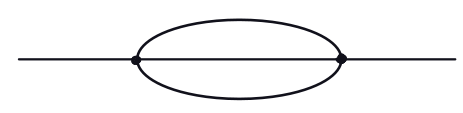
\includegraphics[width=0.3\textwidth]{p2i.png}
      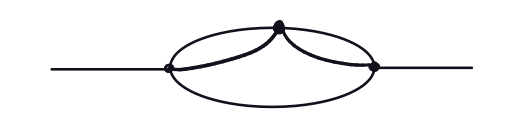
\includegraphics[width=0.3\textwidth]{p2ii.png}
      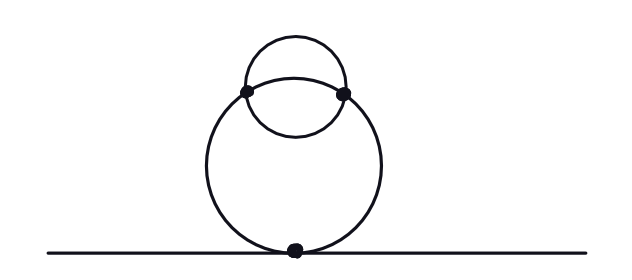
\includegraphics[width=0.3\textwidth]{p2iii.png}
   \end{center}
   \begin{enumerate}[label=(\alph*)]
       \item Obtain the symmetry factor for these Feynman diagrams.
       \item Obtain the amplitude associated to the diagram on the right. Express your result as an integral over the internal momenta.
   \end{enumerate}
\end{problem}
\begin{proof}[Solution]
   Before drawing the diagrams, the vertices of the theory are interchangeable and each contributes with a \(\frac{1}{4!}\) factor, hence the symmetry factor is \(S = \frac{C}{(4!)^V}\) where \(C\) comes from number of ways to draw the diagram starting from empty \(V\) vertices and external legs. To illustrate, we'll draw the Feynman diagram on the left and count for each step. We begin by drawing the external legs and connecting them to one vertex each, yielding a factor of \(4^2\).
   \begin{figure}[H]
      \centering
      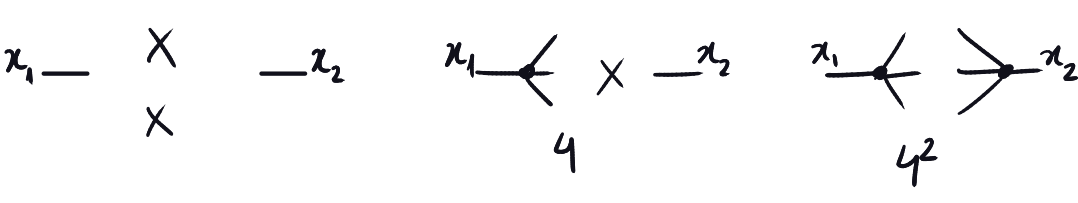
\includegraphics[width=0.8\textwidth]{p2ai.png}
   \end{figure}
   \noindent Now we have \(3!\) ways to connect the internal legs,
   \begin{figure}[H]
      \centering
      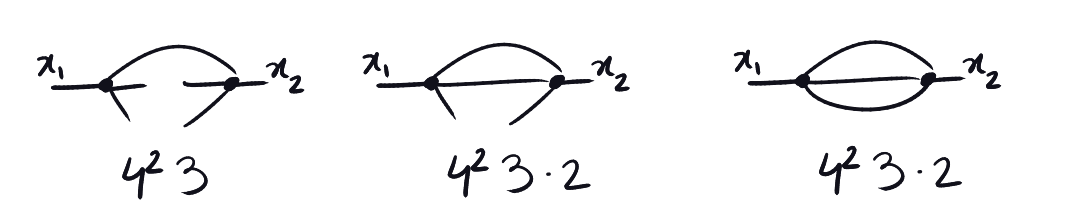
\includegraphics[width=0.8\textwidth]{p2ai2.png}
   \end{figure}
   \noindent and we obtain \(C = 4 (4!),\)  hence \(S = \frac16.\) For the second diagram, we have 
   \begin{figure}[H]
      \centering
      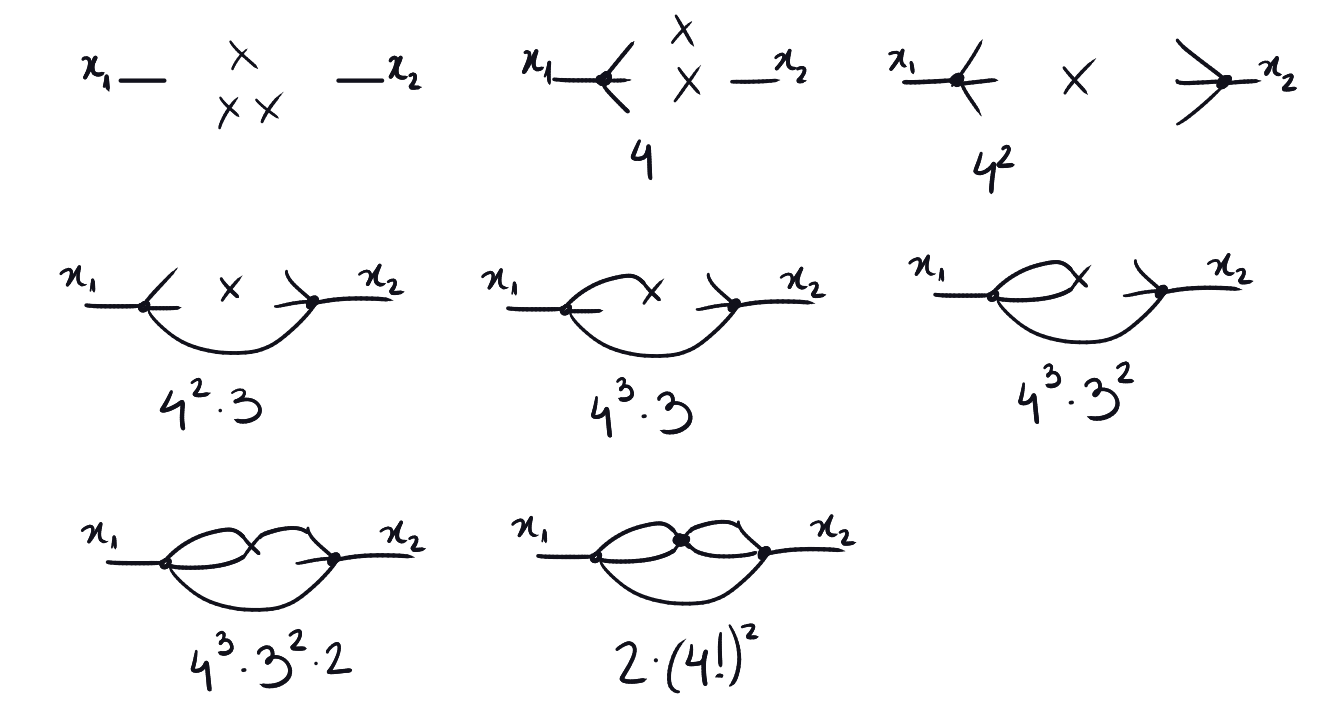
\includegraphics[width=0.8\textwidth]{p2aii.png}
   \end{figure}
   \noindent hence \(S = \frac{2(4!)^2}{(4!)^3} = \frac1{12}.\) For the last diagram, we have
   \begin{figure}[H]
      \centering
      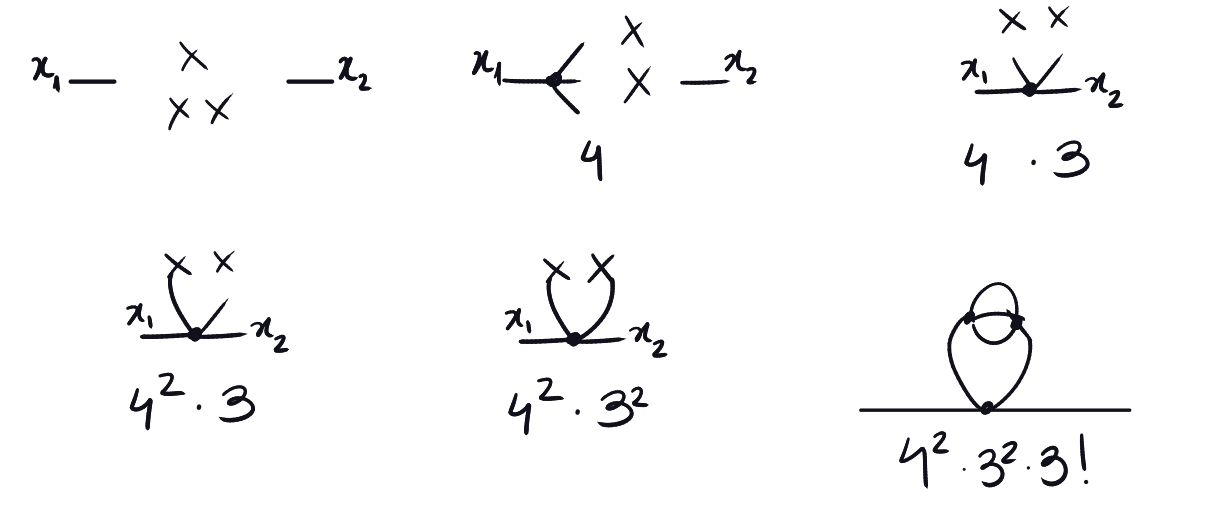
\includegraphics[width=0.8\textwidth]{p2aiii.png}
   \end{figure}
   \noindent hence \(S = \frac{36 \cdot 4!}{(4!)^3} = \frac{1}{16}.\)

   In order to write the momentum conservation terms for the last diagram, we annotate the momenta at each leg
   \begin{figure}[H]
      \centering
      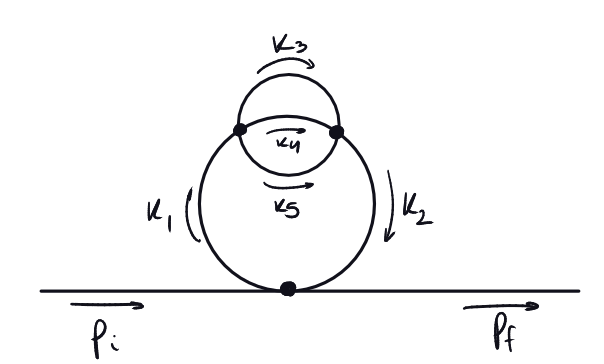
\includegraphics[width=0.5\textwidth]{p2b.png}
   \end{figure}
   \noindent From the Feynman rules, this diagram corresponds to the matrix element
   \begin{align*}
      i \mathcal{M} &= \frac{(-i \lambda)^3}{16(2 \pi)^8 Z_\varphi} \int_{\mathbb{R}^4} \dln4{k_1} \int_{\mathbb{R}^4} \dln4{k_2} \int_{\mathbb{R}^4} \dln4{k_3} \int_{\mathbb{R}^4} \dln4{k_4} \int_{\mathbb{R}^4} \dln4{k_5} \delta(p_i - p_f + k_2 - k_1) \times \\
                    &{}\phantom{=\frac{(-i \lambda)^3}{(2 \pi)^8 S Z_\varphi}} \times \delta(k_1 - k_3 - k_4 - k_5) \delta(k_3 + k_4 + k_5 - k_2) \prod_{\ell = 1}^5 \frac{i}{k_i^2 - m + i \epsilon}
   \end{align*}
   where \(Z_\varphi\) is the coefficient that relates the field with the in and out fields.
\end{proof}
